% Source of the figure p2-outside.pdf: the proof that a common neighbor z of two incomparable elements x, y lies in Q.
% If z is outside Q, it lies in a set Y whose only boundary edges are xz and yz. The minimum sides A_1 minus Y and
% A_2 union Y both contain u and not v, and the red edge xz joins their two differences, which is impossible.
% Compile with pdfLaTeX; the PDF is included in the manuscript at its natural size.
\documentclass[tikz,border=1pt]{standalone}
\usepackage[T1]{fontenc}
\pdfinfoomitdate=1 \pdftrailerid{} \pdfsuppressptexinfo=-1
\definecolor{pathred}{RGB}{200,40,40}
\tikzset{
  vertex/.style={circle, fill=black, inner sep=0pt, minimum size=2.2mm},
  terminal/.style={circle, fill=black, inner sep=0pt, minimum size=3mm},
  edge/.style={line width=0.7pt},
  pathedge/.style={line width=1.8pt, pathred, line cap=round},
  side/.style={rounded corners=8pt, line width=0.7pt, draw=gray!75!black},
  blob/.style={fill=gray!30, draw=gray!70, line width=0.6pt}}
\begin{document}
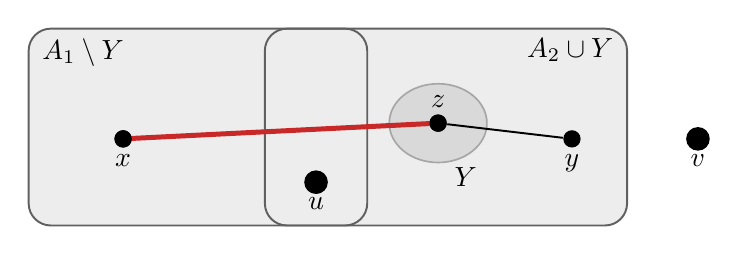
\begin{tikzpicture}[x=1cm, y=1cm]
  \fill[gray!14, rounded corners=8pt] (0,0) rectangle (4.3,2.5);
  \fill[gray!14, rounded corners=8pt] (3.0,0) rectangle (7.6,2.5);
  \draw[side] (0,0) rectangle (4.3,2.5);
  \draw[side] (3.0,0) rectangle (7.6,2.5);
  \node[anchor=north west] at (0.05,2.5) {$A_1 \setminus Y$};
  \node[anchor=north east] at (7.55,2.5) {$A_2 \cup Y$};
  \draw[blob] (5.2,1.3) ellipse (0.62 and 0.5);
  \node at (5.55,0.62) {$Y$};
  \node[vertex] (x) at (1.2,1.1) {};
  \node[vertex] (y) at (6.9,1.1) {};
  \node[vertex] (z) at (5.2,1.3) {};
  \node[terminal] (u) at (3.65,0.55) {};
  \node[terminal] (v) at (8.5,1.1) {};
  \draw[edge] (y) -- (z);
  \draw[pathedge] (x) -- (z);
  \node[vertex] at (x) {};
  \node[vertex] at (z) {};
  \node[below=2pt] at (x) {$x$};
  \node[below=2pt] at (y) {$y$};
  \node[above=2pt] at (z) {$z$};
  \node[below=2pt] at (u) {$u$};
  \node[below=2pt] at (v) {$v$};
\end{tikzpicture}
\end{document}
